%20 min preso!
\documentclass[xcolor=table,english,russian]{beamer}
\usepackage{beamerthemesplit}
\usepackage{wrapfig}
\usetheme{SPbGU}
\usepackage{pdfpages}
\usepackage{amsmath}
\usepackage{mathtools}
\usepackage{cmap}
\usepackage{subcaption}
\usepackage[utf8]{inputenc}
\usepackage[T1, T2A]{fontenc}
\usepackage[]{babel}
\usepackage{indentfirst}
\usepackage{amsmath}
\usepackage{tikz}
\usepackage{multirow}
\usepackage[noend]{algpseudocode}
\usepackage{algorithm}
\usepackage{algorithmicx}
\usepackage{fancyvrb}
\usetikzlibrary{calc}
\usetikzlibrary{shapes,arrows}
\usetikzlibrary{arrows,automata}
\usetikzlibrary{positioning}
\usetikzlibrary{fit}

\usepackage{kbordermatrix} % include package @ document preamble
\renewcommand{\kbldelim}{(} % change default array delimiters to parentheses
\renewcommand{\kbrdelim}{)}

\newcommand\mca{\multicolumn{1}{c}{\cellcolor{red}\textbf{\{a\}}}}
\newcommand\mcb{\multicolumn{1}{c}{\cellcolor{red}\textbf{\{b\}}}}

\usepackage{tabularx}
\newcolumntype{Y}{>{\raggedleft\arraybackslash}X}

\renewcommand{\thealgorithm}{}

\newtheorem{mytheorem}{Theorem}
\renewcommand{\thealgorithm}{}

\newcommand{\tikzmark}[1]{\tikz[overlay,remember picture] \node (#1) {};}
\def\Put(#1,#2)#3{\leavevmode\makebox(0,0){\put(#1,#2){#3}}}

\newcommand{\ltz}{$< 1$}


\tikzset{
    state/.style={
           rectangle,
           rounded corners,
           draw=black, very thick,
           minimum height=2em,
           inner sep=2pt,
           text centered,
           },
}

\beamertemplatenavigationsymbolsempty

\title[Kronecker Product CFPQ]{Поиск путей в графе с КС ограничениями через произведение Кронекера}
%\subtitle[YaccConstructor]{Parsing techniques for graph analysis}
% То, что в квадратных скобках, отображается в левом нижнем углу.
\institute[СПбГУ]{
JetBrains Research, Лаборатория языковых инструментов  \\
Санкт-Петербургский Государственный университет
}

% То, что в квадратных скобках, отображается в левом нижнем углу.
\author[Егор Орачев, Илья Эпельбаум]{Семен Григорьев, Рустам Азимов, Екатерина Шеметова, \\ \textbf{Егор Орачев}, \textbf{Илья Эпельбаум}}

\date{31 Августа 2020}


\begin{document}
{
\begin{frame}[fragile]
  \begin{table}
  \centering
  \begin{tabularx}{\linewidth}{YcX}
    
\includegraphics[height=1.5cm]{pictures/jetbrainsResearch.pdf} \hfill
    & \begin{minipage}[t]{0.3\textwidth}\center \vspace{-1cm}  JBR Interns 2020
      \end{minipage}
    & \hfill 
\includegraphics[height=1.5cm]{pictures/SPbGU_Logo.png}
  \end{tabularx}
  \end{table}
  \titlepage
\end{frame}
}

\begin{frame} \frametitle{Context-Free Path Querying}
  \begin{minipage}[m]{0.45\linewidth}
  \raisebox{-0.5\totalheight}{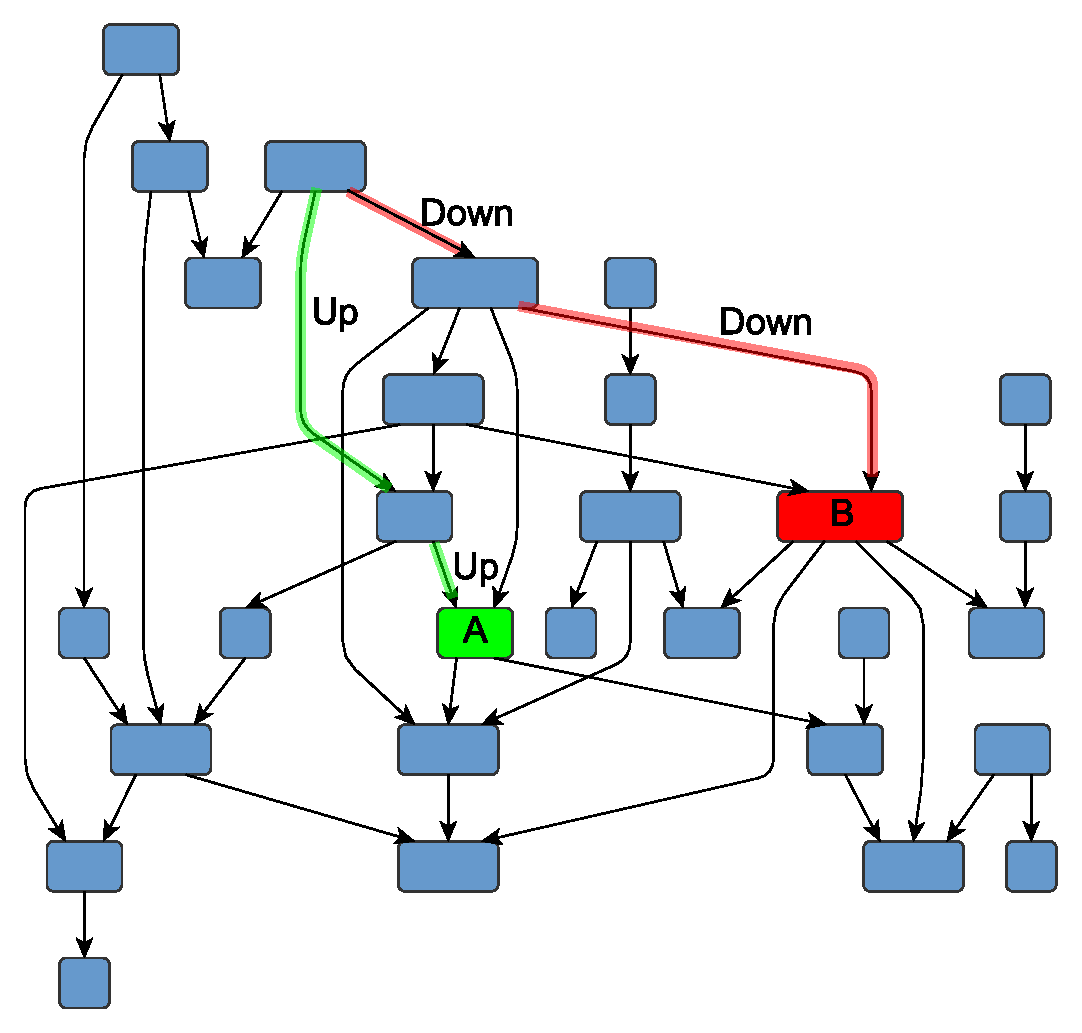
\includegraphics[width=\textwidth]{pictures/hierarchical.pdf}}
  \end{minipage}\hfill
  \begin{minipage}[m]{0.5\linewidth}
  Навигация в графе
  \begin{itemize}
        \item Находятся ли вершины A и B на одном уровне иерархии?
        \item Существует ли путь вида $\textbf{Up}^n \, \textbf{Down}^n$?
        \item Найти все такие пути $\textbf{Up}^n \, \textbf{Down}^n$, которые начинаются в вершине~А
  \end{itemize}
  \end{minipage}
\end{frame}

% \begin{frame}[fragile] \frametitle{Применение}
%     \begin{itemize}
%         \item Статический анализ кода
%         \item Запросы к графовым базам данный
%         \item RDF анализ
%     \end{itemize}
% \end{frame}

\begin{frame}[fragile] \frametitle{CFPQ: Семантика запросов}
    \begin{itemize}
        \item $\mathbb{G} = (\Sigma, N, P)$ --- контекстно-свободная грамматика
        \begin{itemize}
            \item $\Sigma$ конечное множество терминалов
            \item $N$ конечное множество нетерминалов
            \item $P$ конечное множество правил вывода
            \item $L(\mathbb{G},A) = \{ \omega \mid A \Rightarrow^* \omega \}, A \in N$
        \end{itemize}
        %\pause
        \item $G = (V,E,L)$ --- ориентированный граф с метками
        \begin{itemize}
            \item $v \xrightarrow{l} u \in E$
            \item $L \subseteq \Sigma$
        \end{itemize}
        %\pause
        %\item $p = v_0 \xrightarrow{l_0} v_1 \xrightarrow{l_1} \cdots \xrightarrow{l_{n-2}} v_{n-1} \xrightarrow{l_{n-1}} v_n$ --- path in $G$
        \item $\omega(\pi) = \omega(v_0 \xrightarrow{l_0} v_1 \xrightarrow{l_1} \cdots \xrightarrow{l_{n-2}} v_{n-1} \xrightarrow{l_{n-1}} v_n) = l_0 l_1 \cdots l_{n-1}$
        %\pause
        \item $R_A = \{ (n, m) \mid \exists n \pi m$, такой что $\omega(\pi) \in L(\mathbb{G},A)\}, A \in N$
    \end{itemize}
\end{frame}

\begin{frame}[fragile] \frametitle{Существующие решения}
	\begin{itemize}
		\item Решения, основанные на различных техниках парсинга \\ (CYK, LL, LR, etc.)
		%\pause
		\item Решения, основанные на операциях над матрицами
		%\pause
		\item Все существующие решения работают только с КС грамматикой в нормальной форме (Нормальная форма Хомского)
		%\pause
		\item Трансформация требует дополнительного времени на обработку и приводит к \textit{существенному} разрастанию грамматики 
	\end{itemize}
\end{frame}

\begin{frame}[fragile] \frametitle{Рекурсивные автоматы}
    \begin{itemize}
	    \item Представляется набором конечных автоматов (компонент) с дополнительными \textit{рекурсивными вызовами}
	    \item Любая КС грамматика может быть представлена рекурсивным автоматом с одной компонентой на каждый нетерминал 
    \end{itemize}

    \begin{figure}[h]
	    \begin{tikzpicture}[shorten >=1pt,auto]
	        \node[state, initial] (q_0)   {$q_S^0$};
	        \node[state] (q_1) [right=of q_0] {$q_S^1$};
	        \node[state] (q_2) [right=of q_1] {$q_S^2$};
	        \node[state, accepting] (q_3) [right=of q_2] {$q_S^3$};
	    \path[->]
	        (q_0) edge node {a} (q_1)
	        (q_1) edge node {S} (q_2)
	        (q_2) edge node {b} (q_3)
	        (q_1) edge [bend left = 38, above]  node {b} (q_3);
	    \node[draw=black, fit= (q_0) (q_1) (q_2) (q_3), xshift=-4.5ex, inner sep=0.95cm, label=Компонента S] {};
	    \end{tikzpicture}
	    \centering
	    \caption{Рекурсивный автомат для грамматики вида $S \to a S b \mid a b$}
    \end{figure}
\end{frame}

\begin{frame}[fragile] \frametitle{Идея алгоритма}
    \begin{enumerate}
        \item Представить грамматику в виде рекурсивного автомата
        \item Пересечь рекурсивный автомат и граф используя идею классического алгоритма пересечения двух конечных автоматов, описанного в книге Д.Хопкрофта
        \item Использовать транзитивное замыкание, чтобы определить, какие пути выводятся по каким компонентам 
        \item Добавить найденные ребра с нетерминальными метками в граф
        \item Повторять шаги 2 --- 4, пока граф меняется
    \end{enumerate}
\end{frame}

\begin{frame}[fragile] \frametitle{Первая итерация алгоритма}	
    \begin{figure}[h]
    	\centering
    	\begin{subfigure}{.46\textwidth}
    		\begin{center}
    			\begin{tikzpicture}[shorten >=1pt,auto]
    			\node[state] (q_0)                      {$0$};
    			\node[state] (q_1) [right=of q_0]       {$1$};
    			\node[state] (q_2) [right=of q_1]       {$2$};
    			\node[state] (q_3) [right=of q_2]       {$3$};
    			\path[->]
    			(q_0) edge  node {a} (q_1)
    			(q_1) edge  node {S} (q_2)
    			(q_2) edge  node {b} (q_3)
    			(q_1) edge[bend left = 45, above]  node {b} (q_3);
    			\end{tikzpicture}
    		\end{center}
    	\end{subfigure}
        \begin{subfigure}{.07\textwidth}
    	    \begin{center}
    		    \huge{$\otimes$}
    	    \end{center}
        \end{subfigure}
	    \begin{subfigure}{.36\textwidth}
		    \begin{center}
			    \begin{tikzpicture}[shorten >=1pt,auto]
        			\node[state] (q_0)                      {$0$};
        			\node[state] (q_1) [above right=of q_0] {$1$};
        			\node[state] (q_2) [right=of q_0]       {$2$};
        			\node[state] (q_3) [right=of q_2]       {$3$};
        			\path[->]
            			(q_0) edge  node {a} (q_1)
            			(q_1) edge  node {a} (q_2)
            			(q_2) edge  node {a} (q_0)
            			(q_2) edge[bend left, above]  node {b} (q_3)
            			(q_3) edge[bend left, below]  node {b} (q_2);
    			\end{tikzpicture}
		    \end{center}
	    \end{subfigure}
        \begin{subfigure}{.07\textwidth}
	        \begin{center}
	        	\huge{$=$}
	        \end{center}
        \end{subfigure}
        %\pause
	    \begin{subfigure}{.38\textwidth}
		    \begin{center}
    			\[
        		\begin{array}{rcccl}
        		0,0 & \xrightarrow{\text{a}} & 1,1 & & \\
        		0,\underline{\textbf{1}} & \xrightarrow{\textbf{a}} & 1,2 & \xrightarrow{\textbf{b}} & 	3,\underline{\textbf{3}}\\
        		0,2 & \xrightarrow{\text{a}} & 1,0 & & \\
        		2,2 & \xrightarrow{\text{b}} & 3,3 & & \\
        		2,3 & \xrightarrow{\text{b}} & 3,2 & & \\
        		1,3 & \xrightarrow{\text{b}} & 3,2 & & \\
        		\end{array}
        		\]
		    %\caption{Constructing the product automaton}
		    \end{center}
	    \end{subfigure}
        %\pause
        \begin{subfigure}{.08\textwidth}
	        \begin{center}
		        \huge{$$\rightarrow$$}
	        \end{center}
        \end{subfigure}
    	\begin{subfigure}{.48\textwidth}
    		\begin{center}
    			\begin{tikzpicture}[shorten >=1pt,auto]
        			\node[state] (q_0)                      {$0$};
        			\node[state] (q_1) [above right=of q_0] {$1$};
        			\node[state] (q_2) [right=of q_0]       {$2$};
        			\node[state] (q_3) [right=of q_2]       {$3$};
    			    \path[->]
            			(q_0) edge  node {a} (q_1)
            			(q_1) edge  node {a} (q_2)
            			(q_1) edge[color=red, bend left, above]  node {\textbf{S}} (q_3)
            			(q_2) edge  node {a} (q_0)
            			(q_2) edge[bend left, above]  node {b} (q_3)
            			(q_3) edge[bend left, below]  node {b} (q_2);
    			\end{tikzpicture}
    			%\caption{The updated input graph $\mathcal{G}$ using rule $S \to a b$}
    		\end{center}
    	\end{subfigure}
    \end{figure}
\end{frame}


\begin{frame}[fragile] \frametitle{Вторая итерация алгоритма}	
    \begin{figure}[h]
	    \centering
	    \begin{subfigure}{.46\textwidth}
		    \begin{center}
			    \begin{tikzpicture}[shorten >=1pt,auto]
			        \node[state] (q_0)                      {$0$};
    			    \node[state] (q_1) [right=of q_0]       {$1$};
    			    \node[state] (q_2) [right=of q_1]       {$2$};
    			    \node[state] (q_3) [right=of q_2]       {$3$};
    			    \path[->]
            			(q_0) edge  node {a} (q_1)
            			(q_1) edge  node {S} (q_2)
            			(q_2) edge  node {b} (q_3)
            			(q_1) edge[bend left = 45, above]  node {b} (q_3);
    			\end{tikzpicture}			
    		\end{center}
    	\end{subfigure}
	    \begin{subfigure}{.07\textwidth}
		    \begin{center}
			    \huge{$\otimes$}
		    \end{center}
	    \end{subfigure}
	    \begin{subfigure}{.36\textwidth}
		    \begin{center}
			    \begin{tikzpicture}[shorten >=1pt,auto]
        			\node[state] (q_0)                      {$0$};
        			\node[state] (q_1) [above right=of q_0] {$1$};
        			\node[state] (q_2) [right=of q_0]       {$2$};
        			\node[state] (q_3) [right=of q_2]       {$3$};
			    \path[->]
        			(q_0) edge  node {a} (q_1)
        			(q_1) edge  node {a} (q_2)
        			(q_1) edge[bend left, above]  node {\textbf{S}} (q_3)
        			(q_2) edge  node {a} (q_0)
        			(q_2) edge[bend left, above]  node {b} (q_3)
        			(q_3) edge[bend left, below]  node {b} (q_2);
			    \end{tikzpicture}
		    \end{center}
	    \end{subfigure}
        \begin{subfigure}{.07\textwidth}
        	\begin{center}
		        \huge{$=$}
	        \end{center}
        \end{subfigure}
	    %\pause
        \begin{subfigure}{.36\textwidth}
	        \begin{center}
        		\[
        		\begin{array}{rcccccl}
        		0,\underline{\textbf{0}} & \xrightarrow{\textbf{a}} & 1,1 & \xrightarrow{\textbf{S}} & 2,3 & \xrightarrow{\textbf{b}} & 3,\underline{\textbf{2}} \\
        		0,1 & \xrightarrow{\text{a}} & 1,2 & \xrightarrow{\text{b}} &	3,3 & &\\
        		0,2 & \xrightarrow{\text{a}} & 1,0 & & & &\\
        		2,2 & \xrightarrow{\text{b}} & 3,3 & & & &\\
        		1,3 & \xrightarrow{\text{b}} & 3,2 & & & &\\
        		\end{array}
        		\]
	        \end{center}
        \end{subfigure}
        %\pause
        \begin{subfigure}{.07\textwidth}
        	\begin{center}
        		\huge{$$\rightarrow$$}
        	\end{center}
        \end{subfigure}
        \begin{subfigure}{.55\textwidth}
        	\begin{center}
        		\begin{tikzpicture}[shorten >=1pt,auto]
            		\node[state] (q_0)                      {$0$};
            		\node[state] (q_1) [above right=of q_0] {$1$};
            		\node[state] (q_2) [right=of q_0]       {$2$};
            		\node[state] (q_3) [right=of q_2]       {$3$};
        		    \path[->]
                		(q_0) edge  node {a} (q_1)
                		(q_1) edge  node {a} (q_2)
                		(q_1) edge[bend left, above]  node {\text{S}} (q_3)
                		(q_2) edge  node {a} (q_0)
                		(q_2) edge[bend left, above]  node {b} (q_3)
                		(q_3) edge[bend left, below]  node {b} (q_2)
                		(q_0) edge[color=red, bend right = 60, below]  node {\textbf{S}} (q_2);
        		\end{tikzpicture}
        	\end{center}
        \end{subfigure}
    \end{figure}
\end{frame}

\begin{frame}[fragile] \frametitle{Произведение Кронекера}

    \begin{itemize}
        \item \textit{Пересечение} рекурсивного автомата и графа можно выразить через произведение Кронекера
        \item В качесве операндов используются матрицы смежности автомата и графа
    \end{itemize}
	{\scriptsize
	 \renewcommand{\arraystretch}{0.4}
    	$$
    	\begin{pmatrix}
        . & \{a\} & . & .     \\
        . & . & \{S\} & \{b\} \\
        . & . & . & \{b\}     \\
        . & . & . & .
        \end{pmatrix}
        \otimes
        \begin{pmatrix}
        . & \{a\} & . & .     \\
        . & . & \{a\} & .     \\
        \{a\} & . & . & \{b\} \\
        . & . & \{b\} & .
        \end{pmatrix}
        =$$
    }
    {
        \scriptsize
        \renewcommand{\arraystretch}{0.4}
        \setlength\arraycolsep{0.1pt}
        \begin{align*}
        & \kbordermatrix{
        	& (0,0) & (0,1) & (0,2) & (0,3) & \vrule & (1,0) & (1,1) & (1,2) & (1,3) & \vrule &  (2,0) & (2,1) & (2,2) & (2,3) & \vrule &  (3,0) & (3,1) & (3,2) & (3,3) &\\ 
        	(0,0) & . & . & . & . & \vrule & . & \{a\} & . & . & \vrule & . & . & . & . &  \vrule & . & . & . & . \\
        	(0,1) & . & . & . & . & \vrule & . & . & \mca & . & \vrule & . & . & . & . &  \vrule & . & . & . & . \\
        	(0,2) & . & . & . & . & \vrule & \{a\} & . & . & . & \vrule & . & . & . & . &  \vrule & . & . & . & . \\
        	(0,3) & . & . & . & . & \vrule & . & . & . & . & \vrule & . & . & . & . &  \vrule & . & . & . & . \\
        	\hline
        	(1,0) & . & . & . & .  & \vrule & . & . & . & . & \vrule & . & . & . & . & \vrule & . & . & . & . \\
        	(1,1) & . & . & . & .  & \vrule & . & . & . & . & \vrule & . & . & . & . & \vrule & . & . & . & . \\
        	(1,2) & . & . & . & .  & \vrule & . & . & . & . & \vrule & . & . & . & . & \vrule & . & . & . & \mcb \\
        	(1,3) & . & . & . & .  & \vrule & . & . & . & . & \vrule & . & . & . & . & \vrule & . & . & \{b\} & . \\
        	\hline
        	(2,0) & . & . & . & .  & \vrule & . & . & . & . & \vrule & . & . & . & . & \vrule & . & . & . & . \\
        	(2,1) & . & . & . & .  & \vrule & . & . & . & . & \vrule & . & . & . & . & \vrule & . & . & . & . \\
        	(2,2) & . & . & . & .  & \vrule & . & . & . & . & \vrule & . & . & . & . & \vrule & . & . & . & \{b\} \\
        	(2,3) & . & . & . & .  & \vrule & . & . & . & . & \vrule & . & . & . & . & \vrule & . & . & \{b\} & . \\
        	\hline
        	(2,0) & . & . & . & .  & \vrule & . & . & . & . & \vrule & . & . & . & . & \vrule & . & . & . & . \\
        	(2,1) & . & . & . & .  & \vrule & . & . & . & . & \vrule & . & . & . & . & \vrule & . & . & . & . \\
        	(2,2) & . & . & . & .  & \vrule & . & . & . & . & \vrule & . & . & . & . & \vrule & . & . & . & . \\
        	(2,3) & . & . & . & .  & \vrule & . & . & . & . & \vrule & . & . & . & . & \vrule & . & . & . & . \\
        }
        \end{align*}
    }
\end{frame}

\begin{frame}[fragile] \frametitle{Извлечение путей}
    \begin{itemize}
        \item В результате работы алгоритма вычисляется матрица транзитивного замыкания, так называемый \textit{индекс} 
        \item Данная матрица \textit{индекса} может быть использована для извлечения 
        всех путей в графе, которые удовлетворяют достижимости выбранных двух вершин
        \item Поскольку путей потенциально бесконечное количество, фильтрация и \textit{правильная} нумерация существенны для извлечения
    \end{itemize}
\end{frame}

\begin{frame}[fragile] \frametitle{Динамическое транзитивное замыкание}
    \begin{itemize}
        \item \textit{Наивная} версия алгоритма предполагает вычисление транзитивного замыкания на каждой итерации
        \item Транзитивное замыкание \textit{наиболее} сложная часть алгоритма с точки зрения вычислений
        \item Поскольку транзитивное замыкание \textit{дистрибутивно слева}, мы можем разбить матрицу смежности графа на две части: 
        {
            \begin{itemize}
                \item $A$ добавленные ребра
                \item $B$ матрица смежности с прошлой итерации
                \item $M_G = A + B$
                \item $M_{RSM} \otimes M_G = M_{RSM} \otimes A  + M_{RSM} \otimes B$
            \end{itemize}
        }
    \end{itemize}
\end{frame}

\begin{frame}[fragile] \frametitle{Реализация}
    \begin{itemize}
        \item \textit{Наивная} версия алгоритма без динамического транзитивного замыкания на основе библиотеки \textbf{PyGraphBLAS}\footnote{PyGraphBLAS --- python-обертка для SuiteSparse C --- реализации GraphBLAS API для работы с графами в терминах операций линейной алгебры}
        \item Извлечение путей из \textit{индекса} на основе \textbf{PyGraphBLAS}, параметризованное максимальными числом путей для извлечения 
    \end{itemize}
\end{frame}

\begin{frame}[fragile] \frametitle{Замеры}

\end{frame}

\begin{frame}[fragile] \frametitle{Заключение}
    \begin{itemize}
        \item CFQP можно свести к операциям линейной алгебры без трансформации грамматики
        \item Алгоритм применим для RPQ без значительного \textit{overhead}
        \item Индекс, построенный в результате работы алгоритма может быть использован для извлечения \textit{всех} путей
        \item Транзитивное замыкание можно поддерживать за $O(n^3 / log~n)$ 
    \end{itemize}
\end{frame}

\begin{frame}[fragile] \frametitle{Дальнейшие исследования}
  \begin{itemize}
  	\item Исследование проблемы извлечения всех путей (правильная нумерация путей, временные ограничения)
  	\item Детальное сравнение с классическим матричным алгоритмом
  	\item Исследование вычислительной сложности динамического транзитивного замыкания (возможно ли получить субкубическую сложность)
  	\item Реализация алгоритма на GPGPU с использованием разреженных булевых матриц
  	\item Модификация алгоритма для распределенного вычисления 
  	\item Интеграция алгоритма с графовой базой данных (RedisGraph)
\end{itemize}
\end{frame}

\begin{frame} \frametitle{Контакты}
    \begin{itemize}
        \item Семен Григорьев:
        \begin{itemize}
          \item \href{mailto:s.v.grigoriev@spbu.ru}{s.v.grigoriev@spbu.ru}
          \item \href{mailto:Semen.Grigorev@jetbrains.com}{Semen.Grigorev@jetbrains.com}
        \end{itemize}
        \item Рустам Азимов:
        \begin{itemize}
      	    \item \href{mailto:rustam.azimov19021995@gmail.com}{rustam.azimov19021995@gmail.com}
      	    \item \href{mailto:Rustam.Azimov@jetbrains.com}{Rustam.Azimov@jetbrains.com}
        \end{itemize}
        \item Екатерина Шеметова:  \href{mailto:katyacyfra@gmail.com}{katyacyfra@gmail.com}
        \item Егор Орачев: \href{mailto:egor.orachev@gmail.com}{egor.orachev@gmail.com}
        \item Илья Эпельбаум: \href{mailto:iliyepelbaun@gmail.com}{iliyepelbaun@gmail.com}
        \vspace{0.5cm}
        \item Датасет: \href{https://github.com/JetBrains-Research/CFPQ_Data}{https://github.com/JetBrains-Research/CFPQ\_Data}
        \item Реализация алгоритма: \href{https://github.com/YaccConstructor/RedisGraph}{https://github.com/YaccConstructor/RedisGraph}
    \end{itemize}
    \vspace{0.1cm}
\end{frame}

\end{document}
